\chapter{LCD Timings}%
\label{cha:XXXX}

\section{LCD-Timings}%
\label{sec:LCD-Timings}

Because timings for the LCD are important, this chapter shows the measured
timings after the display gets running. The timings needs to be configured by
the \gls{DTS} and are in this way the input for the video DRM driver. The
DRM driver is patched by the Telair International GmbH because of some silicon
errata which belongs to the LCD used in this project (\cite{TI_am335x_errata}).


\subsection{H-Sync timings}%
\label{sub:H-Sync timings}


\begin{figure}[ht]
\begin{center}
    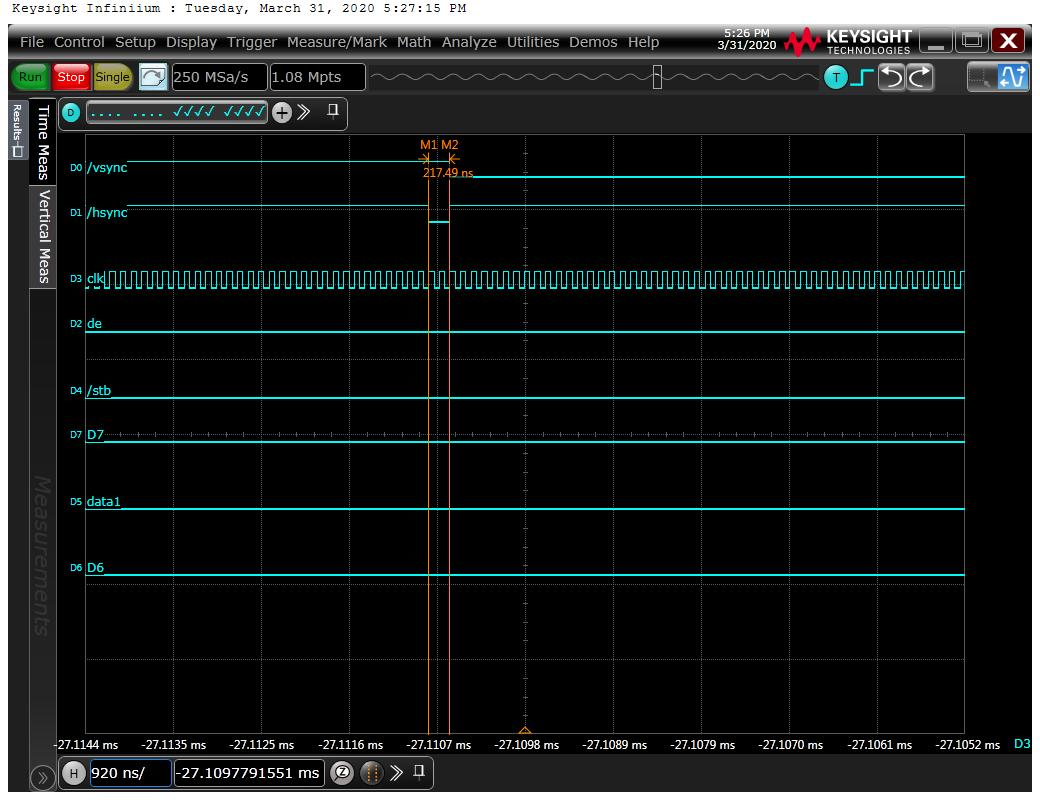
\includegraphics[width=13cm]{pictures/lcd_timings/hsync_length.jpg}
\end{center}
\caption{Length time of one low active H-Sync phase}
\label{fig:hsync_active_time}
\end{figure}



\begin{figure}[ht]
\begin{center}
    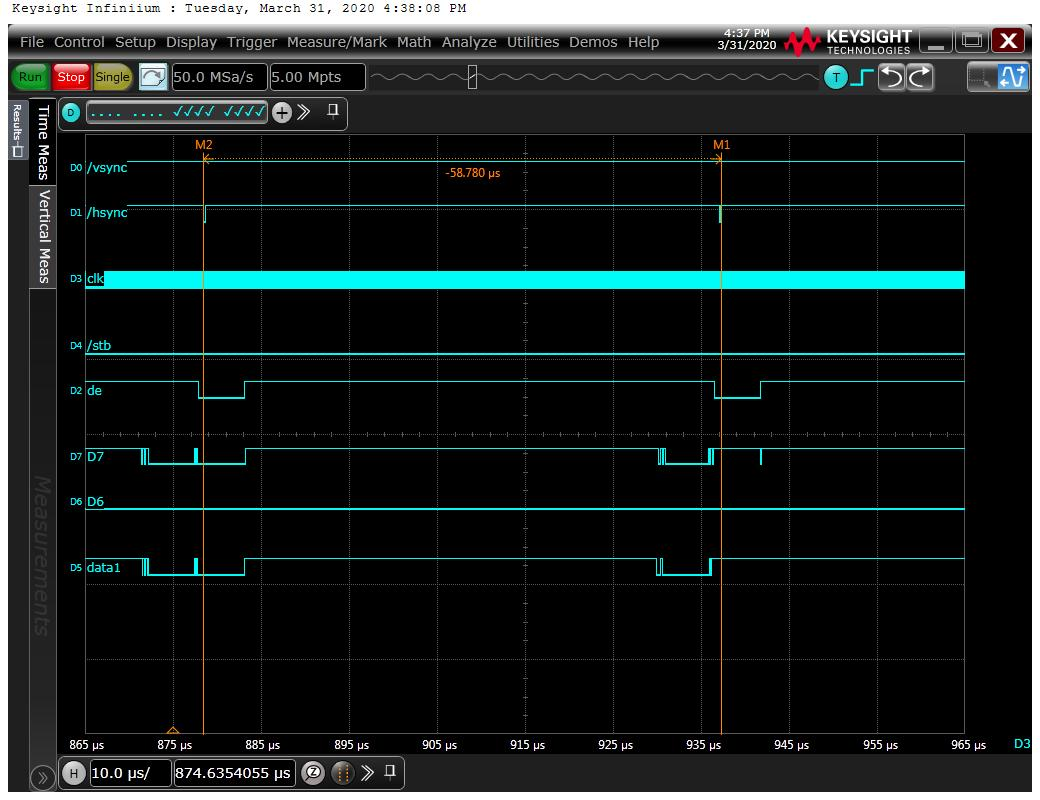
\includegraphics[width=13cm]{pictures/lcd_timings/hsync_periode.jpg}
\end{center}
\caption{Time length of one howl H-Sync period}
\label{fig:hsync_period}
\end{figure}


\subsection{V-Sync timings}%
\label{sub:V-Sync timings}

\begin{figure}[ht]
\begin{center}
    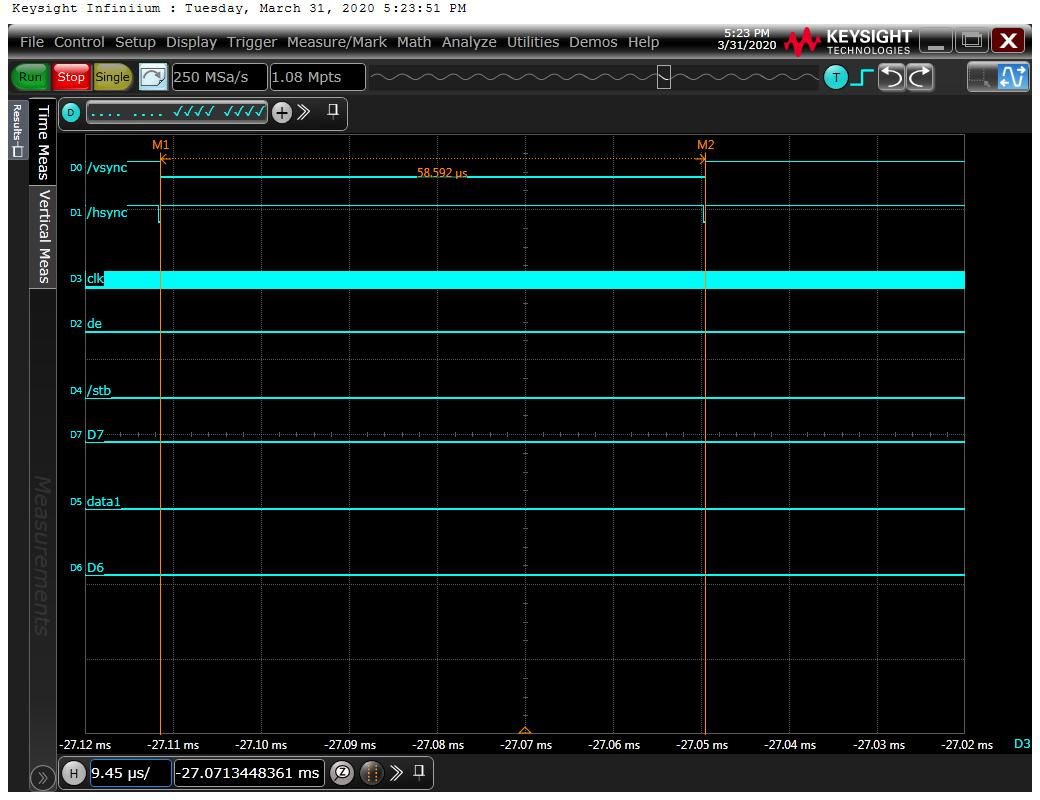
\includegraphics[width=13cm]{pictures/lcd_timings/vsync_length.jpg}
\end{center}
\caption{Length time of one low active V-Sync phase}
\label{fig:vsync_active_time}
\end{figure}


\begin{figure}[ht]
\begin{center}
    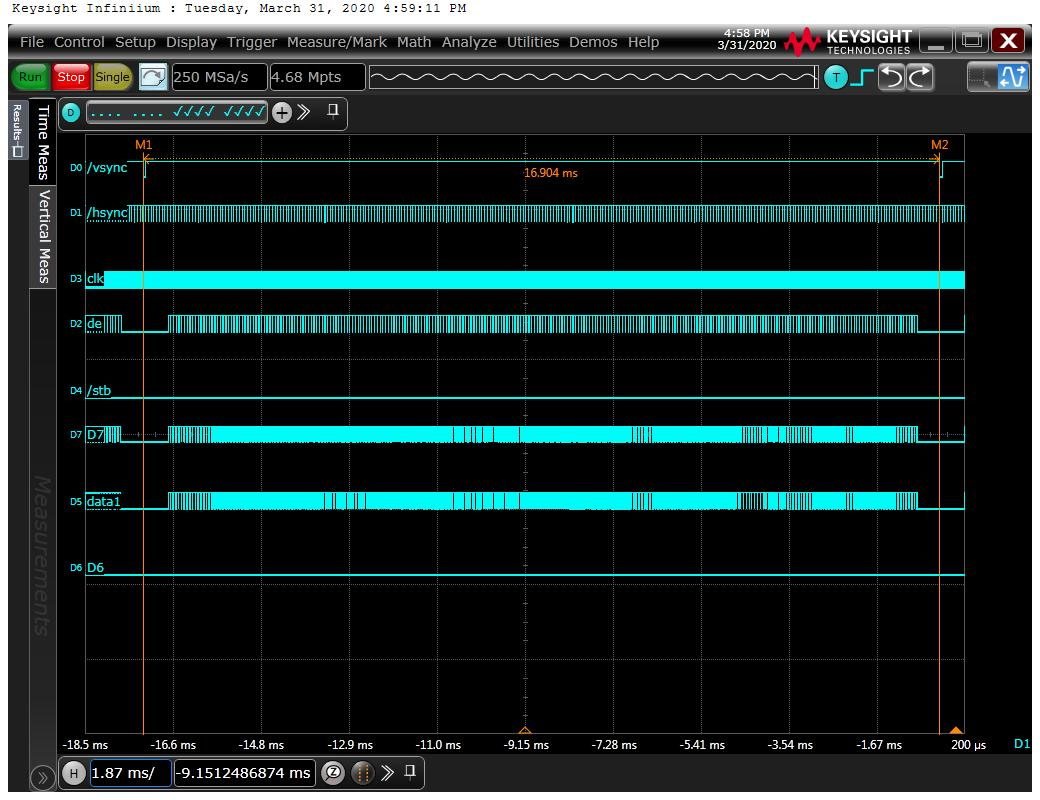
\includegraphics[width=13cm]{pictures/lcd_timings/vsync_periode.jpg}
\end{center}
\caption{Time length of one howl V-Sync period}
\label{fig:one_vsync_period}
\end{figure}



\subsection{One Clock time length}%
\label{sub:Time length one Clock}


\begin{figure}[ht]
\begin{center}
    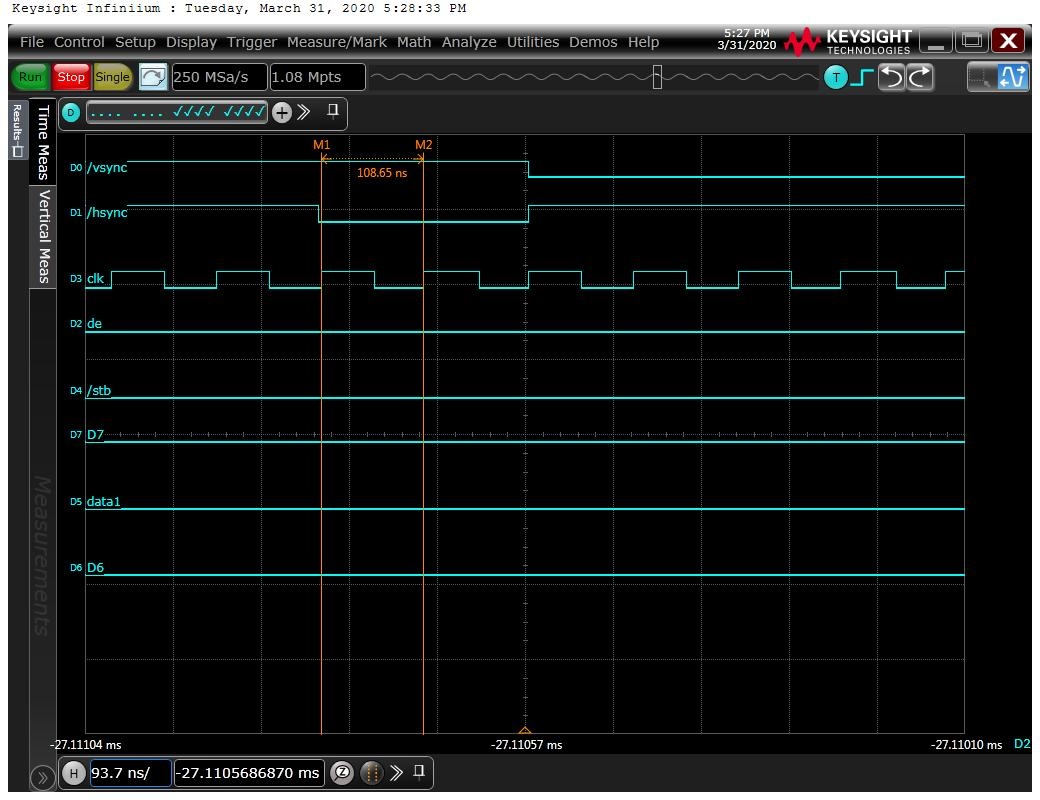
\includegraphics[width=13cm]{pictures/lcd_timings/periode_time_1clk.jpg}
\end{center}
\caption{Time length of one clock period}
\label{fig:one_clock_time}
\end{figure}



\subsection{Other measured LCD timings}%
\label{sub:Other measured LCD timings}

\begin{figure}[ht]
\begin{center}
    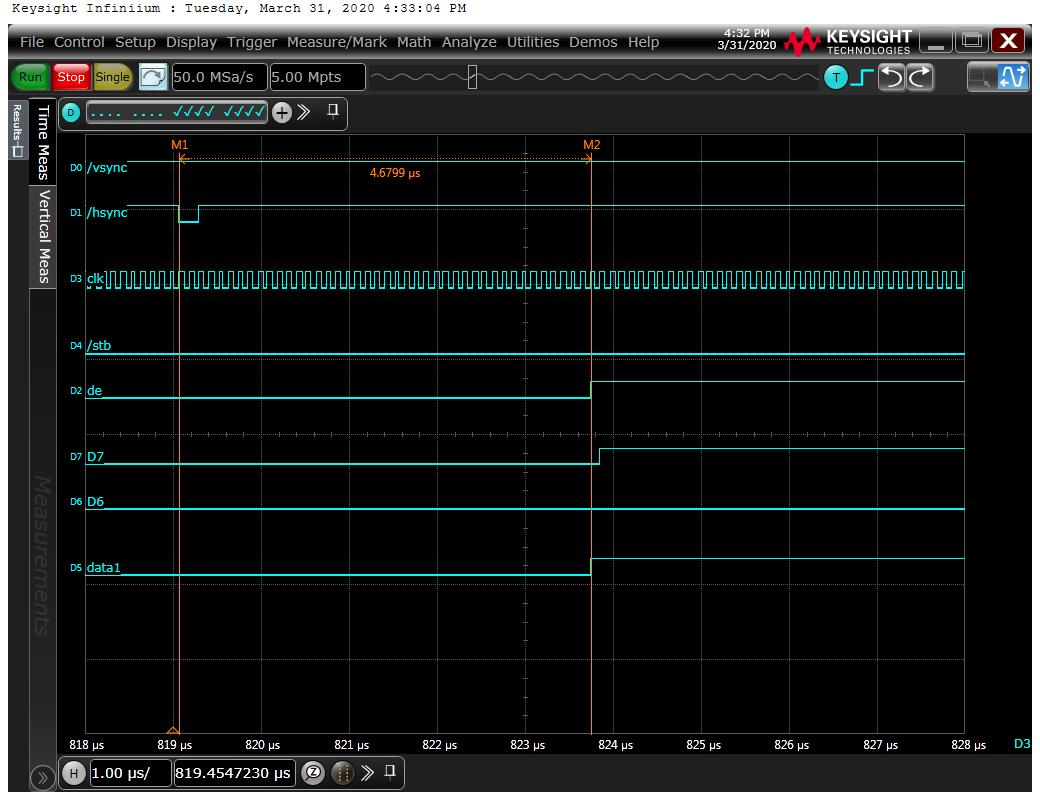
\includegraphics[width=13cm]{pictures/lcd_timings/hsync_falling_de_rising.jpg}
\end{center}
\caption{Time between H-Sync falling edge and DE rising edge}
\label{fig:hsync_de}
\end{figure}
